\section{Proposed Solution: Classic Visitor Pattern}
\label{sec:proposed_solution}

\subsection{Structural Overview}
The Visitor design pattern is strategically proposed to resolve the architectural limitations highlighted in the previous section. It achieves this by extracting the newly required operations from the base class hierarchy and encapsulating them within a distinct ``Visitor'' object. This decoupling ensures that the primary element classes remain relatively stable and strictly adhere to the Open/Closed Principle \cite{gof1994}.

% PLACEHOLDER FOR CLASS DIAGRAM
\begin{figure}[H]
    \centering
    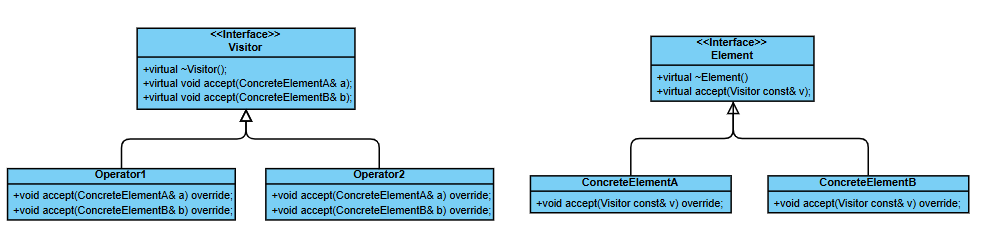
\includegraphics[width=0.7\textwidth]{Figures/assets/ClassicVisitorUML.png}
    \caption{UML Class Diagram of the Classic Visitor Pattern.}
    \label{fig:classic_visitor_diagram}
\end{figure}

\subsection{Conceptual Implementation}
To illustrate the operational flow and the underlying dispatch mechanism, consider the following minimal conceptual implementation. This snippet strips away the business logic to focus entirely on the structural relationship between the \texttt{Visitor} interface and the \texttt{Shape} hierarchy:

\begin{lstlisting}[language=C++, caption=Conceptual implementation illustrating the Visitor structure.]
class Visitor {
public:
    virtual void visit(Circle&) = 0;
    virtual void visit(Rectangle&) = 0;
};

class Shape {
public:
    virtual void accept(Visitor&) = 0;
};

class Circle : public Shape {
public:
    void accept(Visitor& visitor) override {
        // The element passes itself to the visitor
        visitor.visit(*this); 
    }
};
\end{lstlisting}

\subsection{The Core Mechanism: Double Dispatch}
At its core, the Visitor pattern leverages the concept of \textit{Double Dispatch} facilitated by dynamic polymorphism and method overloading. Inherently, C++ only supports \textit{Single Dispatch}, meaning that polymorphic method resolution is based solely on the runtime type of the calling object \cite{iglberger2022}.

The Visitor pattern elegantly circumvents this language limitation by simulating double dispatch through a sequence of two consecutive single dispatch calls, as demonstrated in the conceptual snippet above:
\begin{enumerate}
    \item \textbf{The First Dispatch (Acceptance):} The client invokes the \texttt{accept(Visitor\&)} method on a polymorphic base pointer (e.g., \texttt{Shape*}). Through standard dynamic binding (vtable lookup), the runtime resolves this call to the specific overridden method of the concrete derived class (e.g., \texttt{Circle::accept}).
    \item \textbf{The Second Dispatch (Visitation):} Inside the resolved \texttt{accept} method, the concrete element invokes the \texttt{visit} method on the passed \texttt{Visitor} object, supplying itself (\texttt{*this}) as the argument. At this stage, the compiler uses \textit{overload resolution} (at compile time) to statically bind the call to the appropriate \texttt{visit} signature (e.g., \texttt{visit(Circle\&)}). Then, \textit{virtual dispatch} (at runtime) directs the execution to the corresponding method in the concrete visitor. Thus, the Visitor pattern simulates double dispatch through the combination of compile-time overload resolution and runtime virtual dispatch.
\end{enumerate}
